\subsubsection*{The simplest model}

If the cable is taken as a simple pendulum (lumped mass) of mass $m$ and length $l$ when the boat is towed at a constant speed and constant heading, the equilibrium state of the pendulum is researched.


\begin{figure}[H]
\centering
\psscalebox{0.8 0.8} % Change this value to rescale the drawing.
{
% \usepackage[usenames,dvipsnames]{pstricks}
% \usepackage{epsfig}
% \usepackage{pst-grad} % For gradients
% \usepackage{pst-plot} % For axes
% \usepackage[space]{grffile} % For spaces in paths
% \usepackage{etoolbox} % For spaces in paths
% \makeatletter % For spaces in paths
% \patchcmd\Gread@eps{\@inputcheck#1 }{\@inputcheck"#1"\relax}{}{}
% \makeatother
% % User Packages:
% \usepackage{amsmath}
% \usepackage{amsfonts}
% \usepackage{amssymb}
% \usepackage{algorithm}
% \usepackage{algorithmic}
% 
\psscalebox{1.0 1.0} % Change this value to rescale the drawing.
{
\begin{pspicture}(0,-2.5449028)(7.8730617,2.5449028)
\definecolor{colour0}{rgb}{0.015686275,0.17254902,0.6666667}
\definecolor{colour1}{rgb}{0.19215687,0.80784315,0.07058824}
\psline[linecolor=black, linewidth=0.04](3.9089148,1.8969576)(5.087519,1.8969576)
\psline[linecolor=black, linewidth=0.04](4.3086305,1.8825132)(2.4941862,-0.9530424)
\psline[linecolor=black, linewidth=0.02, arrowsize=0.05291667cm 2.0,arrowlength=1.4,arrowinset=0.0]{->}(2.4910214,-0.9562069)(2.1720343,-1.4675993)
\psline[linecolor=black, linewidth=0.02, arrowsize=0.05291667cm 2.0,arrowlength=1.4,arrowinset=0.0]{->}(2.5062113,-0.9815234)(3.0176039,-1.3106374)
\psline[linecolor=red, linewidth=0.03, arrowsize=0.05291667cm 2.0,arrowlength=1.4,arrowinset=0.0]{->}(2.4634843,-0.9416389)(0.6248878,-0.9416389)
\psline[linecolor=black, linewidth=0.03, arrowsize=0.05291667cm 2.0,arrowlength=1.4,arrowinset=0.0]{->}(2.4712036,-0.94421196)(2.4712036,-2.5091243)
\psline[linecolor=colour0, linewidth=0.03, arrowsize=0.05291667cm 2.0,arrowlength=1.4,arrowinset=0.0]{->}(2.4749463,-0.9205862)(2.4819639,0.6092383)
\psarc[linecolor=black, linewidth=0.03, linestyle=dashed, dash=0.17638889cm 0.10583334cm, dimen=outer, showpoints=true, arrowsize=0.05291667cm 2.0,arrowlength=1.4,arrowinset=0.0]{<-}(4.3055897,1.8829225){0.5368421}{239.0}{360.0}
\pscircle[linecolor=colour1, linewidth=0.04, fillstyle=solid,fillcolor=colour1, dimen=outer](2.4808948,-0.9663335){0.14177215}
\rput[bl](5.136343,1.3518596){$\theta$}
\rput[bl](2.9794803,-1.2677482){$\vec{u_{\theta}}$}
\rput[bl](1.7402645,-1.4873561){$\vec{u_{r}}$}
\rput[bl](0.0,-0.8332749){$\vec{F_{fluid}}$}
\rput[bl](2.0186048,0.35742274){$\vec{\Pi}$}
\rput[bl](2.5953488,-2.5449028){$\vec{w}$}
\psline[linecolor=black, linewidth=0.012](4.3382597,2.3725133)(4.142704,1.9058465)
\psline[linecolor=black, linewidth=0.012](4.1752973,2.3725133)(3.9797416,1.9058466)
\psline[linecolor=black, linewidth=0.012](4.990112,2.3725133)(4.794556,1.9058466)
\psline[linecolor=black, linewidth=0.012](4.8271494,2.3725133)(4.6315937,1.9058466)
\psline[linecolor=black, linewidth=0.012](4.664186,2.3725133)(4.4686303,1.9058466)
\psline[linecolor=black, linewidth=0.012](4.501223,2.372513)(4.3056674,1.9058465)
\psline[linecolor=black, linewidth=0.012](5.1530747,2.372513)(4.9575195,1.9058465)
\rput[bl](3.2064939,-0.22996545){$(m,l)$}
\psline[linecolor=black, linewidth=0.04, arrowsize=0.05291667cm 2.0,arrowlength=1.4,arrowinset=0.0]{->}(5.5277476,2.0859988)(7.966104,2.0859988)
\rput[bl](6.5798025,2.2449028){$\vec{v_c}$}
\end{pspicture}
}


}
\caption{Representation of cable as a simple pendulum}
\label{fig:model_pendulum}
\end{figure}


$\vec{w}$ is the gravitational force and $\vec{\Pi}$ represent the Archimedes principle, $\vec{F_{fluid}}$ is the resistance due to the fluid and $\vec{T}$ is the force of the base on the cable. $\vec{v_c}$ is the speed of the base (e.g.\ the boat) and $(m,l)$ is the mass and length of the pendulum. If the system is at equilibrium then the speed of the cable is the same as the speed of the base. 

%\begin{align}
\begin{equation}
 \vec{0} = \vec{T}+\vec{F_{fluide}}+\vec{w}+\vec{\Pi}\\
 \label{equ_Stab_1}
\end{equation}


Where if $C_D$ is the drag coefficient $\rho$ is the fluid density, $r$ is the radius of the cable:


{
\begin{align}
\centering
\vec{F_{fluide}} &= -C_D (2 r l) \rho \frac{ \|v_c\|}{2} \cdot \vec{v_c} \\
\vec{w} &= m \cdot \vec{g} \\
\vec{\Pi} &= - \rho \pi r^2 l \cdot \vec{g}
\end{align}
}
If~\ref{equ_Stab_1} is projected on $\vec{u_{\theta}}$ to get rid off the unknown force $\vec{T}$ the result is:

\begin{equation}
 0 = (m g - l \rho \pi r^2 g) \cdot \sin(\theta)-C_D l 2 r \rho \frac{v_c^2}{2} \cdot \cos(\theta)\\
 \label{equ_Stab_2}
\end{equation}

Thus, the angle $\theta$ can be found if the cable is more heavy enough ($m -l \rho \pi r^2 > 0)$ i.e.\ the cable is more dense than the fluid otherwise the cable should be always on the surface:

\begin{equation}
 \theta = \arctan(\frac{C_D l 2 r \rho}{2 g \cdot (m - l \rho \pi r^2)} \cdot v_c^2)\\
 \label{equ_theta_1}
 \end{equation}
 
With this formula the depth of the end of the pendulum can be computed with different parameters, linear mass of the cable \ref{fig:depth_mass_speed_pendulum} or the length of the cable depending 
 
 \begin{figure}[H]
\centering
    \begin{minipage}[b]{0.4\textwidth}
    \centering
    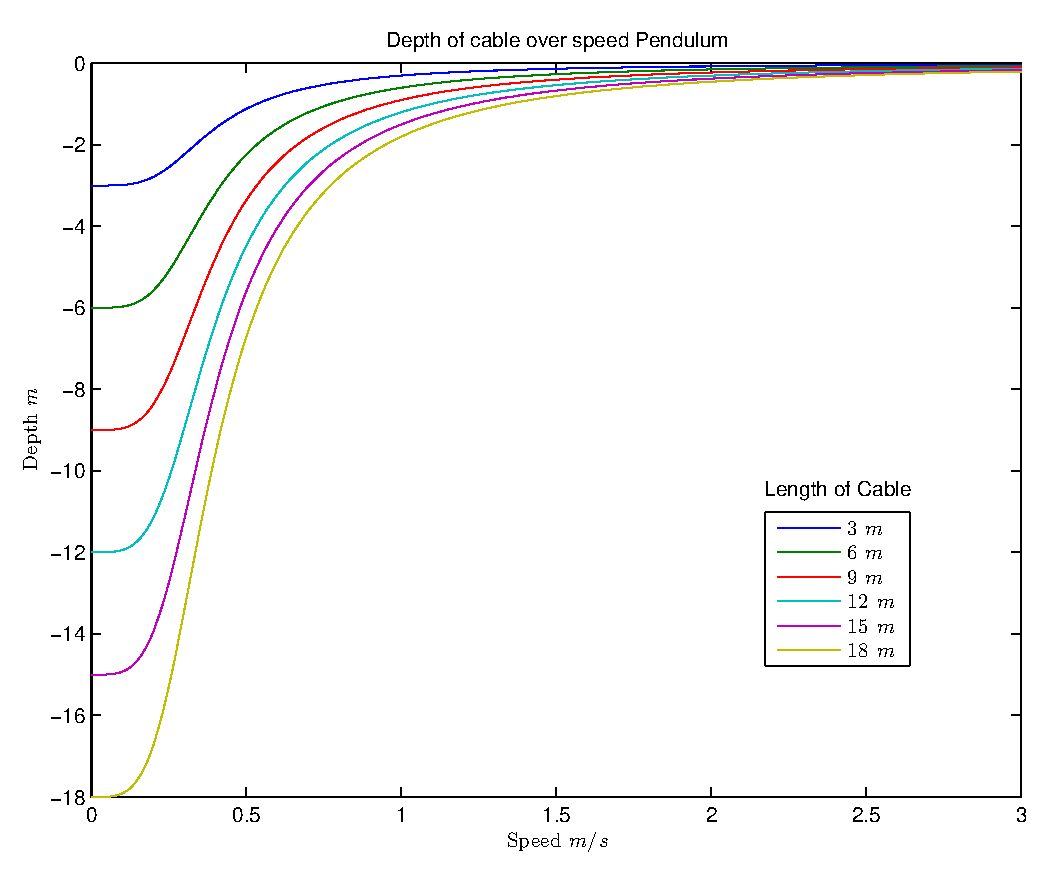
\includegraphics[scale=0.4,angle=0]{depth_length_speed_pendulum}
    \caption{Profile of Depth over Speed of base depending on length of the cable.}
    \label{fig:depth_length_speed_pendulum}
    \end{minipage}
    \hfill
    \begin{minipage}[b]{0.4\textwidth}
    \centering
    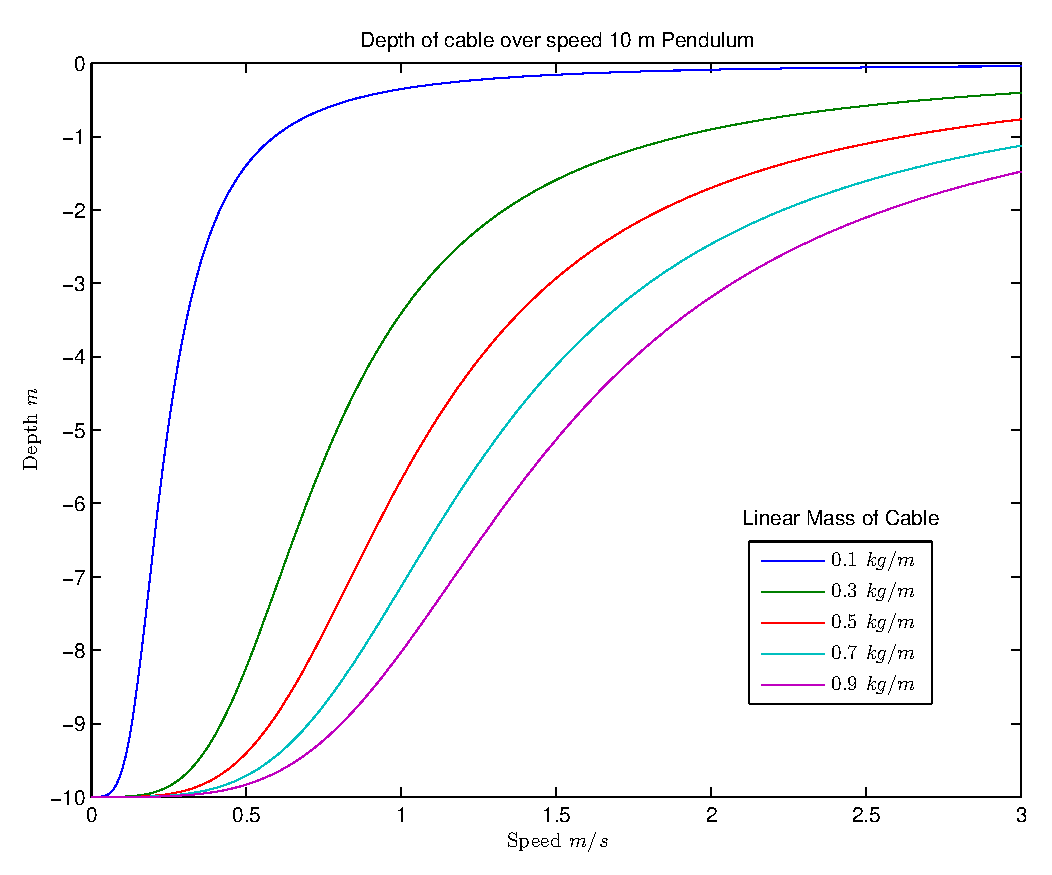
\includegraphics[scale=0.4,angle=0]{depth_mass_speed_pendulum}
    \caption{Profile of Depth over Speed of base depending on linear mass of the cable.}
    \label{fig:depth_mass_speed_pendulum}
    \end{minipage}
\end{figure}

The present model is developed using the work by Vegar Johansen PhD thesis~\cite{johansen2007modelling} as a basis, in this model the rods are modelled by vectors and centres of gravity and allows the application of different forces on the cable, in this model the fluid friction is added.

A rod can be characterised by the two following object:

\begin{figure}[H]
\centering
\psscalebox{0.5 0.5} % Change this value to rescale the drawing.
{
% \usepackage[usenames,dvipsnames]{pstricks}
% \usepackage{epsfig}
% \usepackage{pst-grad} % For gradients
% \usepackage{pst-plot} % For axes
% \usepackage[space]{grffile} % For spaces in paths
% \usepackage{etoolbox} % For spaces in paths
% \makeatletter % For spaces in paths
% \patchcmd\Gread@eps{\@inputcheck#1 }{\@inputcheck"#1"\relax}{}{}
% \makeatother
% % User Packages:
% \usepackage{amsmath}
% \usepackage{amsfonts}
% \usepackage{amssymb}
% \usepackage{algorithm}
% \usepackage{algorithmic}
% 
\psscalebox{1.0 1.0} % Change this value to rescale the drawing.
{
\begin{pspicture}(0,-2.4740124)(6.1989417,2.4740124)
\definecolor{colour0}{rgb}{0.50980395,0.50980395,0.50980395}
\rput(0.025257645,-2.4567273){\psaxes[linecolor=black, linewidth=0.04, tickstyle=top, axesstyle=axes, labels=none, ticks=none, dx=1.0cm, dy=1.0cm]{->}(0,0)(0,0)(2,2)}
\psline[linecolor=black, linewidth=0.04, arrowsize=0.05291667cm 2.0,arrowlength=1.4,arrowinset=0.0]{->}(0.018941855,-2.456201)(1.1663103,-1.6140957)
\psline[linecolor=black, linewidth=0.04, dotsize=0.07055555cm 2.0]{*-*}(3.092626,2.270115)(4.2399945,-0.43514836)
\psline[linecolor=colour0, linewidth=0.02, arrowsize=0.05291667cm 2.0,arrowlength=1.4,arrowinset=0.0]{->}(0.00841554,-2.456201)(3.0189419,2.2280095)
\psline[linecolor=colour0, linewidth=0.02, arrowsize=0.05291667cm 2.0,arrowlength=1.4,arrowinset=0.0]{->}(0.039994486,-2.4456747)(4.1663103,-0.47725362)
\psline[linecolor=colour0, linewidth=0.02, arrowsize=0.05291667cm 2.0,arrowlength=1.4,arrowinset=0.0]{->}(0.039994486,-2.4667273)(3.6505208,0.9332727)
\rput[bl](3.861047,0.90169376){$r$}
\rput[bl](3.6189418,-0.96146417){$c$}
\rput[bl](2.1663103,1.6174833){$a$}
\psline[linecolor=black, linewidth=0.02, arrowsize=0.05291667cm 2.0,arrowlength=1.4,arrowinset=0.0]{->}(4.1978893,2.4701147)(5.3452578,-0.23514834)
\rput[bl](4.818942,1.4385358){$b = c-a$}
\end{pspicture}
}


}
\caption{Representation of $r$ and $b$.}
\label{fig:draw_ref_rb}
\end{figure}

\begin{align}
r &= \begin{bmatrix}
    r_x \\
    r_y \\
    r_z
\end{bmatrix}\, \textnormal{is the center of gravity}\\
b &= \begin{bmatrix}
    b_x \\
    b_y \\
    b_z
\end{bmatrix}\, \textnormal{is the vector for the rod orientation}
\end{align}

The forces acting on the cable are applied on the ends of each rods, meaning for example, the gravity force would be split in two forces acting on each side of the bar. Leading to the base formulas where a and c are the extremity of the bar, $f_X$ is the force applying at the point $X$ and $L$ is the length of the rod :

\begin{align}
\ddot{r} &= \dfrac{1}{m}  (f_a+f_c) \\
\ddot{b} &=  \dfrac{6}{m}(f_a+f_c) - \dfrac{b}{L^{2}}  (\dfrac{6}{m}b^{T}(f_a+f_c)+\dot{b}^{T}\dot{b}) 
\end{align}



Then the model adds the use of the Baumgarte stabilization constraint~\cite{baumgarte1972stabilization} to respect the physical constraint on the bar , length and position of fixed points if there is. 
The stabilization technique is a PID method therefore it depends on coefficient parameters, in a variable-step solver augmenting the P an D coefficient improve the simulation but will increase the time needed to do the simulation.

Johansen proposes three scenarios for this model, a free cable, a fixed-free scenario where one side of the cable is attached to a point and the last one is a fixed-fixed where both side are attached to points.
The model interesting for the modelling of the sailboat towing a cable is the fixed-free scenario where the attachment point is the boat.

The external forces acting on each of the rods of the cable model are the gravitational force ($\vec{P}$) and the fluid friction ($\vec{f}_{fluid}$) and the Archimedes principle ($\vec{\Pi}$), each rod is considered a cylinder : for the rod $n$ :

{
\begin{align}
\begin{split}
\vec{P} &= m \vec{g}  \\
F_{fluid~n,a,x} &= -\frac{C_D (2 r ) \rho}{2} \cdot \displaystyle \int_{0}^{L/2} v_{a,x}(l)^2 \cdot \frac{2l}{L} \, \mathrm{d}l\  \\
\vec{v_{a}}(l) &= \vec{\dot{r_n}} - \frac{2 l}{L} \cdot \vec{b_n} \times \frac{\vec{\dot{b_n}}}{L} \nonumber \\
\vec{v_{c}}(l) &= \vec{\dot{r_n}} + \frac{2 l}{L} \cdot \vec{b_n} \times \frac{\vec{\dot{b_n}}}{L} \nonumber\\
\vec{\Pi} &= - \rho \pi L r^2 \vec{g} \label{equ_archi}
\end{split}
\end{align}
}
In~\ref{equ_archi}  $S$  it the surface of the cable and $C_D$ the drag coefficient for a cylinder, $\rho$ the density of the fluid, $r$ is the radius of the cable , $L$ the length of the rod.

The term $\frac{2 l}{L}$ in the integral part is there to compensate the lever effect when applying this force on the extremity of the rod.



\begin{figure}[H]
\centering
    \begin{minipage}[b]{0.4\textwidth}
    \centering
    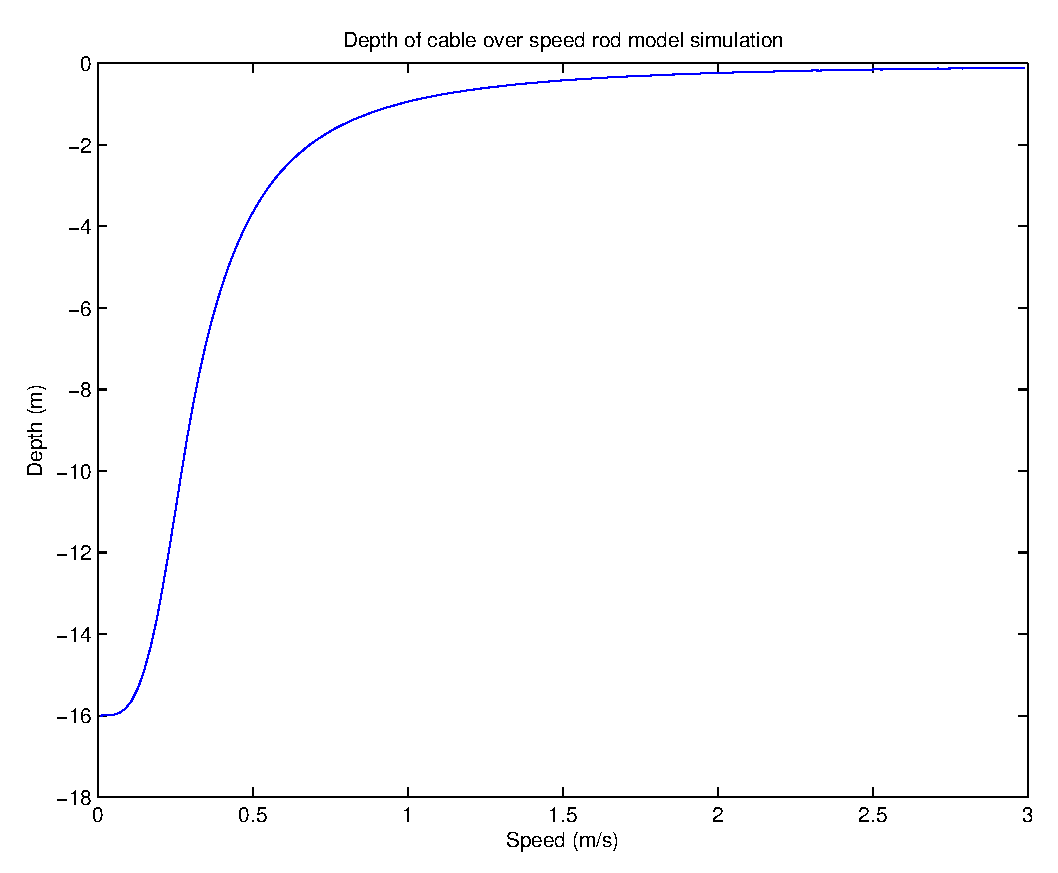
\includegraphics[scale=0.45,angle=0]{depth_speed_rcm}
    \caption{Depth of the cable when stabilized at the final speed.}
    \label{fig:depthIndSpeed}
    \end{minipage}
    \hfill
    \begin{minipage}[b]{0.45\textwidth}
    \centering
    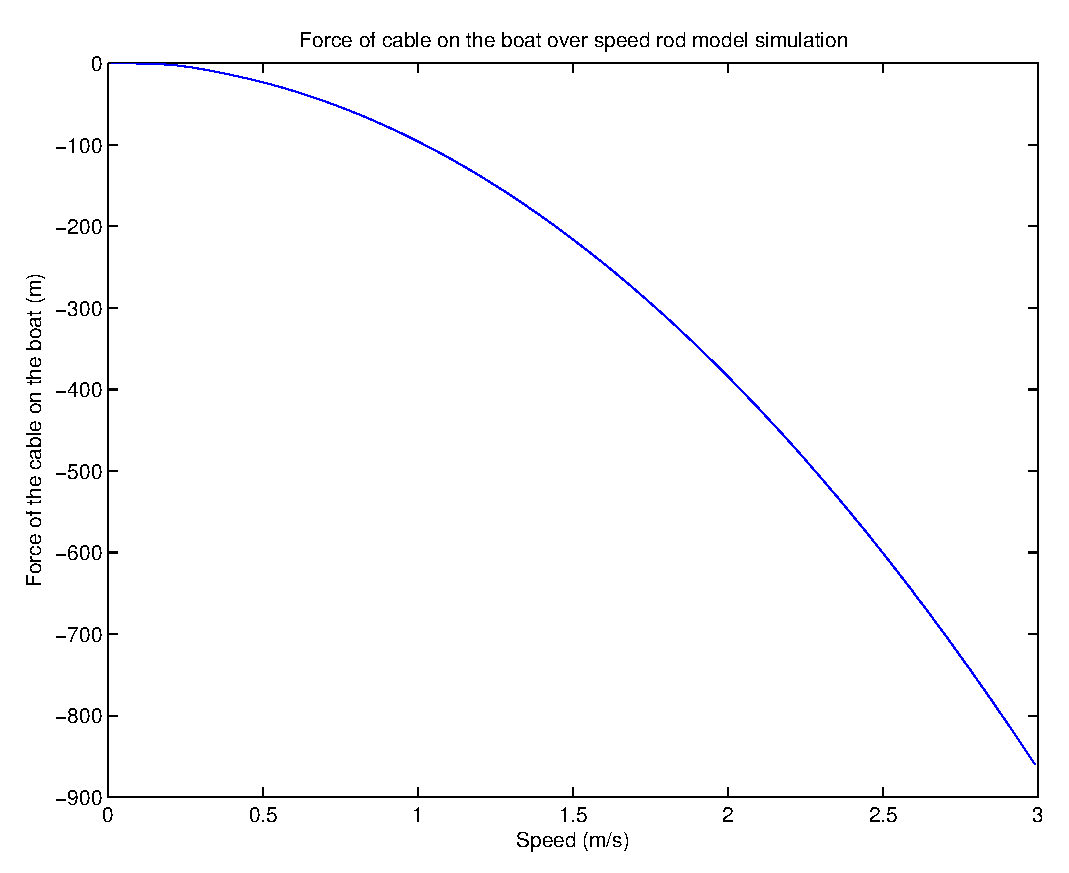
\includegraphics[scale=0.45,angle=0]{force_speed_rcm}
    \caption{Force of the cable on the boat when stabilized at the final speed.}
    \label{fig:forceIndSpeed}
    \end{minipage}
\end{figure}

In figure~\ref{fig:depthIndSpeed} is represented the angle of the cable to the vertical depending of the speed of the boat when the system is stabilized. The curve follows the equation \label{equ_theta_1}.
It means beyond a certain velocity the cable will be useless due to be not enough submerged and horizontal. The simulation at equilibrium respect the equation of the pendulum.

In figure~\ref{fig:forceIndSpeed} is the reaction of the cable on the boat, a constant for the vertical reaction and a decrease following a square law for the horizontal reaction dependent on the fluid friction force.


\begin{figure}[H]
\centering
    \begin{minipage}[b]{0.4\textwidth}
    \centering
    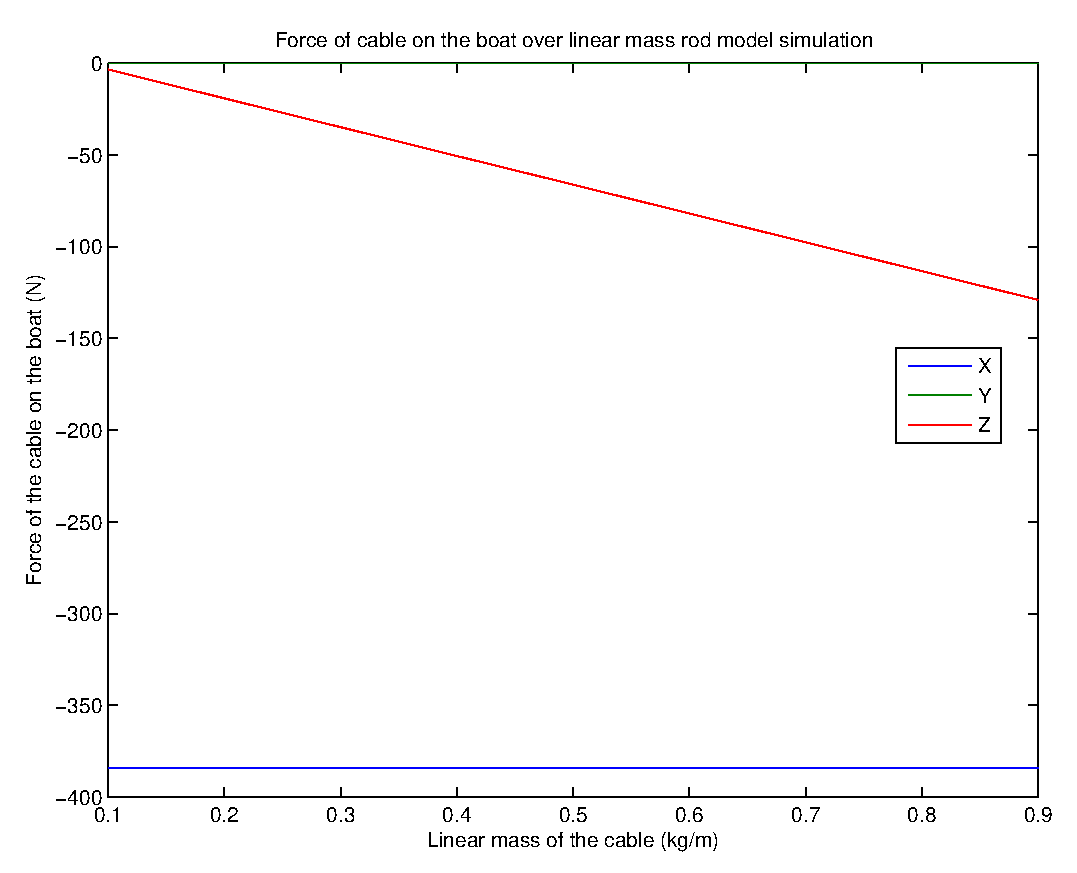
\includegraphics[scale=0.45,angle=0]{force_mass_rcm}
    \caption{Variation of reaction force of cable on boat depending on linear  mass of cable.}
    \label{fig:massForce}
    \end{minipage}
    \hfill
    \begin{minipage}[b]{0.45\textwidth}
    \centering
    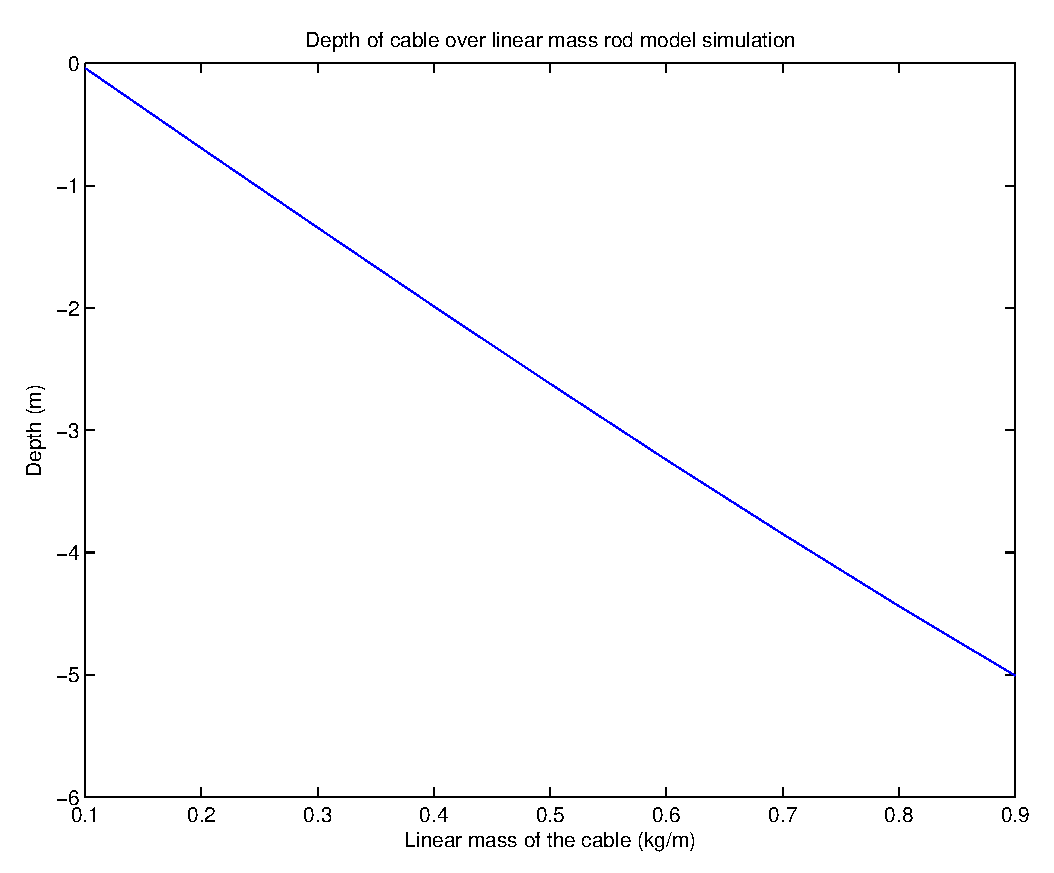
\includegraphics[scale=0.45,angle=0]{depth_mass_rcm}
    \caption{Variation of the depth of the cable depending on the linear mass of cable.}
    \label{fig:linmassAngle}
    \end{minipage}
\end{figure}

\begin{equation}
 \vec{0} = \vec{f}_{cable/boat}+\vec{f}_{fluid}+\vec{P}+\vec{\Pi}\\
 \label{equ_Stab}
\end{equation}

In figure~\ref{fig:massForce} is represented the force of the cable on the boat once stabilized and depending of the mass of the last rod. The horizontal force is constant over mass, this is logical as when stabilized mass does not appear in the horizontal part of the equation \eqref{equ_Stab}. And as for the vertical reaction it varies linearly with the mass, thus corresponding to the precedent equation on the vertical axis.

Changing the linear mass or the mass of the last rod have different effect on the final angle of the cable(see~\ref{fig:linmassAngle}), the errors can be reduced by changing the coefficient of the Baugmarte stabilization but it will influence on the computation time when using a variable-step solver.

This model include a tolerance to errors which are resolved by the Baumgarte stabilisation technique but there still some left over:


\begin{figure}[H]
\centering
    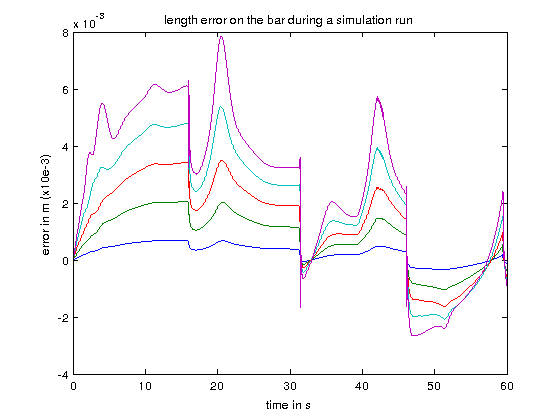
\includegraphics[scale=0.5,angle=0]{error_length_run.png}
    \caption{Error in length of the rods during a simulation run.}
    \label{fig:errorLRod}
\end{figure}

In the figure~\ref{fig:errorLRod} the error in length reach a maximum around one centimetre for a rod length of four meters\footnote{To see simulations : \href{https://www.youtube.com/watch?v=T7DRGq3E5x8}{Fixed cable video https://www.youtube.com/watch?v=T7DRGq3E5x8} or \href{https://www.youtube.com/watch?v=V4X0PsgsXZY}{Moving cable with a constant speed video https://www.youtube.com/watch?v=V4X0PsgsXZY}}, this error can be considered negligible in this case but in some runs if the start is too sharp then, the simulation may diverge.

To simulate this model there is more than one options, but to not make it diverge tweaking must be made.
If using a fixed-step size integration (Runge-Kutta) the step need to be $\sim\mathcal{O}(10^{-3})$, it is the limit of this method and if the cable endure big acceleration it will diverge.

With a solver with variable step-size (ODE45) the result will be in general more accurate but the computation time became very high needing more than one second to compute one second of simulation.If possible Matlab coder should be used to help improve the computation time.